\documentclass[a4paper,11pt,hidelinks]{book}

    \usepackage[utf8]{inputenc}
    \usepackage{lipsum}     % uso \lipsum per creare corpo di testo
    \usepackage{geometry}   % aggiusta i margini delle pagine
    \usepackage{hyperref}   % trasforma l'indice in un ipertesto
    \usepackage{color}      % aggiunge i colori
    \usepackage{multicol}   % posso usare le multicolonne
    \usepackage{amssymb}
    \usepackage{amsmath}
    \usepackage{amsthm}
    \usepackage{tikz}
    \usepackage{blindtext}
    \usepackage{fancyref}
    \usepackage{mdframed}
    


% =====================================
\usetikzlibrary{shapes,arrows,chains}


\tikzstyle{rounded square} = [rectangle, rounded corners, text centered, draw=black]
\tikzstyle{line} = [draw, -latex']


\tikzstyle{arrow} = [thick,->,>=stealth]

% =====================================

\theoremstyle{definition}
\newtheorem*{definizione}{Definizione}

% =====================================
\title{Linguaggi di programmazione - (04138)
    \\ cdlt Informatica - Unibo}
\author{Alberto Zuccari}
\date{A.A. 2022 - 2023}
% =====================================

\renewcommand*\contentsname{Indice} % denominazione dell'indice


% #################################################################

\begin{document}

\maketitle

\tableofcontents

\chapter{Macchine astratte}

\section{macchine astratte e linguaggi}

    \subsection{Macchina Astratta}

    Prendiamo come esempio iniziale la \textbf{macchina di von Neumann} è una struttura molto semplice ma allo stesso tempo molto flessibile e con tante varianti.
    
    La macchina esegue un ciclo ripetitivo (\textbf{FDE})
    
    I programmi e i dati sono indistinguibili e risiedono nella memoria interna
    \begin{center}
    \textcolor{red}{\textit{\textbf{Una macchina esiste per eseguire il suo linguaggio}}}
    \end{center}
    Linguaggio e macchina esistono in simbiosi ma:
    \begin{itemize}
        \item Una macchina corrisponde ad un linguaggio (il suo)
        \item Un Linguaggio può essere eseguito da più macchine \\
            (il linguaggio C può essere eseguito da macchine diverse)
    \end{itemize}
    
    \begin{definizione}[$\mathcal{MA}$]\label{MA}
    Una Macchina Astratta è un insieme di strutture dati ed algoritmi in grado di memorizzare ed eseguire programmi. L'interprete è un componente essenziale.
    \end{definizione}
    
    \subsection{Interprete}
    È il componente che \textit{interpreta} le istruzioni.
    dentro ha varie operazioni e strutture dati che gli permettono di:
    
    \begin{table}[h]
        \centering
        \begin{tabular}{|c|c|}
        \hline
        elaborare i dati primitivi & controllo e sfruttamento dell'ALU \\ \hline
        controllare la sequenza di & incremento del PC;  \\ 
        esecuzione delle operazioni & Salti \\ \hline
        controllare il trasferimento dei dati & gestione dei metodi di indirizzamento \\ \hline
        gestire la memoria & indirizzamento e trasferimento dei blocchi\\
    \hline
        \end{tabular}
        \label{Operazioni interprete}
    \end{table}
    
    \subsection{Linguaggio Macchina}
    \begin{definizione}[$\mathcal{L_M}$]\label{LM}
    Linguaggio macchina di $\mathcal{M}$. \\ È il linguaggio che è compreso dall'interprete di $\mathcal{M}$.
    \end{definizione}
    
    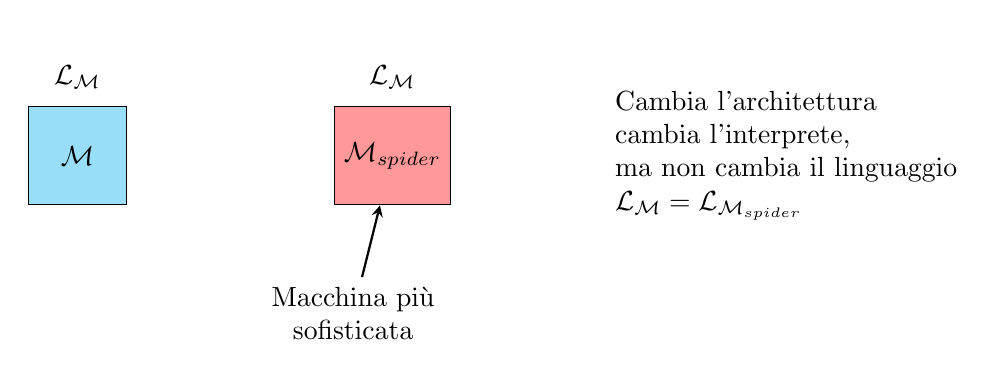
\begin{tikzpicture}[node distance=1cm]
    
        <TikZ code>
        \node (a) [rectangle, minimum width=1.25cm, minimum height=1.25cm] {$\mathcal{L_M}$};
        \node (b) [rectangle, below of=a, minimum width=1.25cm, minimum height=1.25cm, draw=black, fill=cyan!40] {$\mathcal{M}$};
        
        \node (c) [rectangle, right of=a, xshift=3cm, minimum width=1.25cm, minimum height=1.25cm] {$\mathcal{L_M}$};
        \node (d) [rectangle, right of=b, xshift=3cm, minimum width=1.25cm, minimum height=1.25cm, draw=black, fill=red!40]{$\mathcal{M}_{spider}$};
        
        \node[align=left] (punto) at (9,-1) {Cambia l'architettura \\ cambia l'interprete, \\ ma non cambia il linguaggio \\ $\mathcal{L_M} = \mathcal{L}_{\mathcal{M}_{spider}}$ \par};
        
        \node (S) [below of=d, yshift=-1cm, xshift=-0.5cm, align=center] {Macchina più \\ sofisticata \par};
        
        \draw [arrow] (S) -- (d);
        
    \end{tikzpicture}

    \subsection{Microprogrammazione}
    \begin{multicols}{2}
    La microprogrammazione ha lo scopo di far condividere a calcolatori \textit{diversi} (lenti ed economici o veloci ma costosi) lo stesso insieme di istruzioni e \textbf{avere quindi lo stesso linguaggio macchina}.
    
    Nel caso di simulazione mediate microprogrammi si parla di \textit{emulazione} e il livello della microprogrammazione è detto \textit{firmware}.
    
    Una macchina microprogrammata costituisce un primo esempio di \textit{gerarchia} di due macchine astratte.

    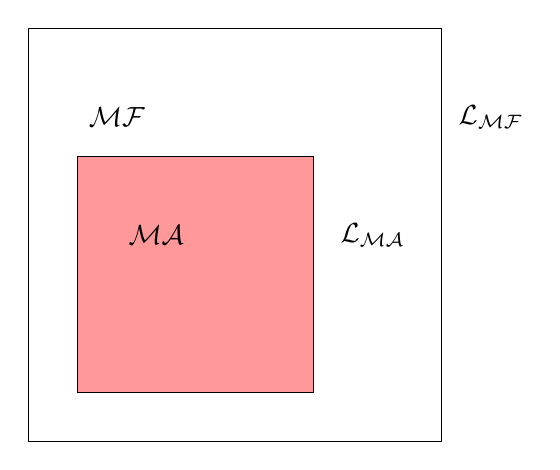
\begin{tikzpicture}[node distance=1cm]
    
        <tikZ code>
        \node (MF) [rectangle, minimum width=5.25cm, minimum height=5.25cm, draw=black] {};
        \node (MAPF) [rectangle, minimum width=3cm, minimum height=3cm, xshift=-0.5cm, yshift=-0.5cm, draw=black, fill=red!40] {};
        
        \node (MFt) [xshift=-1.5cm, yshift=1.5cm] {$\mathcal{MF}$};
        \node (MAPFt) [xshift=-1cm] {$\mathcal{MA}$};
        \node (LMF) [xshift=3.25cm, yshift=1.5cm] {$\mathcal{L_{MF}}$};
        \node (LMAPF) [xshift=1.75cm] {$\mathcal{L_{MA}}$};
    
    \end{tikzpicture}

    \end{multicols}

    \subsection{Realizzazione di una macchina astratta}
    Una qualsiasi macchina astratta $\mathcal{M_L}$ per essere effettivamente realizzata deve essere:
    
    \begin{multicols}{2}
    
    \begin{itemize}
        \item realizzata in \textcolor{orange}{\textbf{hardware}} \label{realizzare HW} \\
        Utilizzare qualche dispositivo fisico per eseguire le istruzioni di $\mathcal{L}$ 
        
        \vspace{0.41cm}

        Con questo possiamo:

        \begin{tabular}{|c|}
        \hline
            usarla solo per macchine \\ di basso livello   \\ \hline
            avere una velocità massima \\ \\ \hline
            non abbiamo flessibilità, \\ c'è solo il linguaggio $\mathcal{L}$ \\ \hline
        \end{tabular}
        
        
        
        \item emulata (o simulata) via \textcolor{orange}{\textbf{firmware}} \label{emulare via FW} \\
        Utilizzare microprogrammi (scritti in un linguaggio $\mathcal{L}'$) per la creazione di strutture dati e algoritmi. 
        

        Facendo ciò avremmo:
        
        \begin{tabular}{|c|}
        \hline
            una macchina ospite \\ microprogrammabile \\ \hline
            un'alta velocità \\ \\ \hline
            un'alta flessibilità. \\ \\ \hline
        \end{tabular}
    \end{itemize}
    
    \end{multicols}
    
    \newpage
    
    \begin{itemize}
        \item Interpretata o simulata via \textcolor{orange}{\textbf{software}} \label{simulata via SW} \\
        Le strutture dati e gli algoritmi della macchina astratta $\mathcal{MA}$ sono realizzate mediate programmi scritti nel linguaggio della macchina ospite $\mathcal{MO}$.
        
        \vspace{0.5cm}
        
        \centering
        \begin{tabular}{|c|}
        \hline
        macchina ospite qualsiasi \\ \\ \hline
        minore velocità \\ \\ \hline
        massima flessibilità \\ \\
        \hline
        \end{tabular}
        
    \end{itemize}

\section{gerarchie di macchine astratte e di linguaggi}
    Un'architettura informatica si struttura in una serie di macchine astratte gerarchiche

    \begin{multicols}{2}

    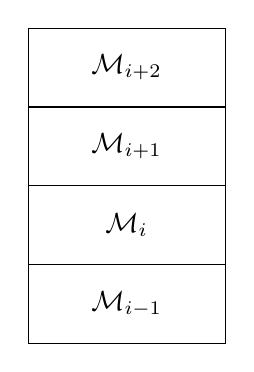
\begin{tikzpicture}[node distance=1cm]
        <TikZ code>
        
        \node (1) [rectangle, minimum width=2.5cm, minimum height=1cm, draw=black] {$\mathcal{M}_{i+2}$};
        \node (2) [rectangle, below of=1, minimum width=2.5cm, minimum height=1cm, draw=black] {$\mathcal{M}_{i+1}$};
        \node (3) [rectangle, below of=2, minimum width=2.5cm, minimum height=1cm, draw=black] {$\mathcal{M}_{i}$};
        \node (4) [rectangle, below of=3, minimum width=2.5cm, minimum height=1cm, draw=black] {$\mathcal{M}_{i-1}$};
    \end{tikzpicture}
    
    
        $\mathcal{M}_i$ \\
        Utilizza i servizi forniti da chi sta sotto $( \mathcal{M}_{i-1} )$ ovvero il linguaggio $\mathcal{L_M}_{i-1}$ \\
        per fornire servizi a chi sta sopra $( \mathcal{M}_{i+1} )$

    \end{multicols}
    
    \begin{center}
    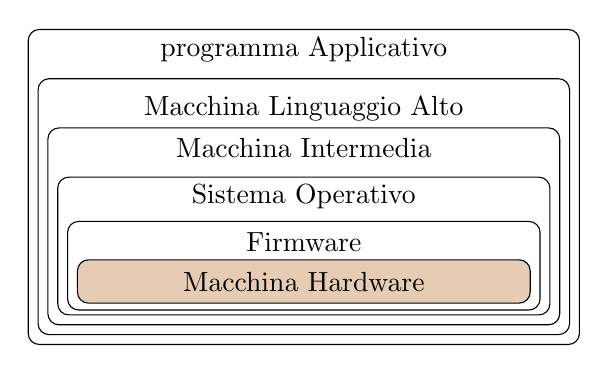
\begin{tikzpicture}[node distance=0.5cm]\label{gerarchia canonica}
        
        <TikZ codeZ>
        
            \node (PA) [rounded square, minimum width=7cm, minimum height=4cm,] { };
            \node (PAt) [above of=PA, yshift=1.25cm] {programma Applicativo};
            \node (MLAL) [rounded square, minimum width=6.75cm, minimum height=3.25cm, yshift=-0.25cm] { };
            \node (MLALt) [above of=MLAL, yshift=0.75cm] {Macchina Linguaggio Alto};
            \node (MI) [rounded square, minimum width=6.5cm, minimum height=2.5cm, yshift=-0.5cm] { };
            \node (MIt) [above of=MI, yshift=0.5cm] {Macchina Intermedia};
            \node (SO) [rounded square, minimum width=6.25cm, minimum height=1.75cm, yshift=-0.75cm] { };
            \node (SOt) [above of=SO, yshift=0.125cm] {Sistema Operativo};
            \node (F) [rounded square, minimum width=6cm, minimum height=1.125cm, yshift=-1cm] { };
            \node (Ft) [above of=F, yshift=-0.2cm] {Firmware};
            \node (HW) [rounded square, minimum width=5.75cm, minimum height=0.55cm, yshift=-1.2cm, fill=brown!40] { };
            \node (HWt) [above of=HW, yshift=-0.5cm] {Macchina Hardware};
        
    \end{tikzpicture}
    \end{center}
    
    \newpage
    
    
    \mdfsetup{%
    middlelinecolor=red,
    middlelinewidth=2pt,
    backgroundcolor=red!10,
    roundcorner=10pt}
    
    \begin{mdframed}
    
    \section{Preliminari e notazione}
        Dobbiamo fare prima un preambolo:
        \begin{definizione}[Funzione]
            $f:A\longrightarrow B$ \\
            È una corrispondenza tra elementi di A e di B. La funzione $f$ a ogni elemento $a\in A$ associa un solo elemento $b\in B$.
        \end{definizione}
        \begin{definizione}[Funzione \textcolor{red}{\textit{parziale}}]
            $f:A \longmapsto B$ \\
            È una corrispondenza che \textit{può} essere \textcolor{red}{non definita} su qualche $a \in A$
        \end{definizione}
        \begin{definizione}[Programma sequenziale]
            $\mathcal{P}_r^\mathcal{L}$ \\
            Indica un programma $\mathcal{P}_r$ scritto nel linguaggio $\mathcal{L}$ \\
            A $\mathcal{P}_r^\mathcal{L}$ è associata una funzione \textcolor{red}{\textbf{parziale}} $\mathcal{P^L}$ (parziale perché se non viene definito un input il programma non termina, quindi può non essere definita su qualche $a \in A$) sull'insieme dei dati che rappresenta la \textcolor{red}{semantica} del programma $\mathcal{P}_r^\mathcal{L}$
            \[\mathcal{P^L}:\mathcal{D} \longrightarrow \mathcal{D}\]
            \[\mathcal{P^L}(Input)=(Output)\]
        \end{definizione}
        \subsubsection{Esempio: semantica di un programma sequenziale}
            Prendiamo un frammento di programma sequenziale: 
        
        \begin{center}
        \begin{tabular}{l l l}
            $\mathcal{P}_r^\mathcal{L}=$ & \verb|read(x);| & \\
             & \verb|If(x == 1)| & \verb|then print(x)| \\
             & & \verb|else while true do skip;| \\
        \end{tabular}
        \end{center}
        E la sua \textbf{semantica} come funzione da input ad output\\
        \(\mathcal{P^L}(x)=1 \textnormal{ se } x=1, \textnormal{ indefinita alteimenti}\)  \\
        \verb| |
        
    \end{mdframed}
    
    \newpage
    
    \mdfsetup{%
    middlelinecolor=red,
    middlelinewidth=2pt,
    backgroundcolor=yellow!25,
    roundcorner=10pt}
    
    \begin{mdframed}
    \section{Come leggere quelle robe strane}
    
    \vspace{0.25cm}
    \(\textcolor{red}{\mathcal{I}^{\mathcal{L}o}{_{\mathcal{L}1}}} = \)
    Un interprete scritto in $\mathcal{L}o$ che esegue programmi scritti in $\mathcal{L}1$
    \flushleft
    La macchina ospite è $\mathcal{M}_{\mathcal{L}o}$, mentre la macchina astratta realizzata su di essa dall'interprete è $\mathcal{M}_{\mathcal{L}1}$
    
    \vspace{0.25cm}
    \( \textcolor{red}{\mathcal{I}^{\mathcal{L}o}{_{\mathcal{L}1}}(\mathcal{P}^{\mathcal{L}1}, x)} = \)
    risultato del calcolo del programma $\mathcal{P}$ (scritto in $\mathcal{L}1$ con $x$ come dato in input
    
    \vspace{0.25cm}
    \( \textcolor{red}{\mathcal{I}^{\mathcal{L}o}{_{\mathcal{L}1}}(\mathcal{I}^{\mathcal{L}1}{_{\mathcal{L}2}}(\mathcal{P}^{\mathcal{L}2}, x))} = \)
    risultato del calcolo di $\mathcal{P}$ scritto in $\mathcal{L}2$ con $x$ come input 
    
    \flushleft
    La macchina ospite è $\mathcal{M}{_{L}o}$, sulla quale è realizzata una macchina intermedia $\mathcal{M}{_{L}1}$, grazie al primo interprete, mentre la macchina astratta $\mathcal{M}{_{L}2}$, attraverso il secondo interprete, è in grado di eseguire il programma $\mathcal{P}$. 
    
    \vspace{0.25cm}
    \( \textcolor{red}{\mathcal{C}^{\mathcal{L}o}{_{\mathcal{L}1, \mathcal{L}2}}} = \)
    un compilatore scritto in $\mathcal{L}o$ che traduce programmi scritti in $\mathcal{L}1$ in equivalenti programmi scritti in $\mathcal{L}2$ 
    
    \vspace{0.25cm}
    \( \textcolor{red}{\mathcal{I}^{\mathcal{L}o}{_{\mathcal{L}1}}(\mathcal{C}^{\mathcal{L}1}{_{\mathcal{L}2, \mathcal{L}3}}, \mathcal{P}^{\mathcal{L}2}) = \mathcal{P}1^{\mathcal{L}3}} \)
    cioè l'interprete eseguito sulla macchina ospite $\mathcal{ML}o$, realizza la macchina astratta $\mathcal{M}_{\mathcal{L}1}$ ed esegue un compilatore, scritto in $\mathcal{L}1$ che traduce il programma $\mathcal{P}$ scritto in $\mathcal{L}2$ in un equivalente programma $\mathcal{P}1$ (scritto in $\mathcal{L}3$)
    
    \end{mdframed}
    
    \newpage
    
\section{Implementare un linguaggio: interpreti e compilatori}
    Scartiamo la 1° opzione (realizzare in \textcolor{orange}{\textbf{hardware}} (\ref{realizzare HW})) e utilizziamo le altre due
    % \begin{multicols} {2}
    \begin{itemize}
        \item \textcolor{orange}{\textbf{Software}}
        \item \textcolor{orange}{\textbf{Firmware}}
    \end{itemize}
    % \end{multicols}
    Dati:
    \begin{itemize}
        \item Un linguaggio $\mathcal{L}$ da implementare
        \begin{itemize}
            \item ovvero per il quale realizzare una macchina astratta $\mathcal{M_L}$
        \end{itemize}
        \item Una macchina astratta $\mathcal{M}o_{\mathcal{L}o}$ (macchina ospite)
        \begin{itemize}
            \item col suo linguaggio $\mathcal{L}o$
        \end{itemize}
    \end{itemize}
    Vogliamo
    \begin{itemize}
        \item Implementare $\mathcal{L}$ su $\mathcal{M}o_{\mathcal{L}o}$
    \end{itemize}
    Abbiamo \textbf{2} modi radicalmente diversi per farlo.

    \subsection{Implementazione interpretativa pura}\label{Implementazione interpretativa pura}
    Per realizzare la macchia astratta $(\mathcal{M_L})$ per il linguaggio $(\mathcal{L})$ dobbiamo scrivere un \textcolor{red}{\textit{interprete}} per $\mathcal{L}$ su $\mathcal{M}o_{\mathcal{L}o}$
    
    \vspace{0.5cm}
    
    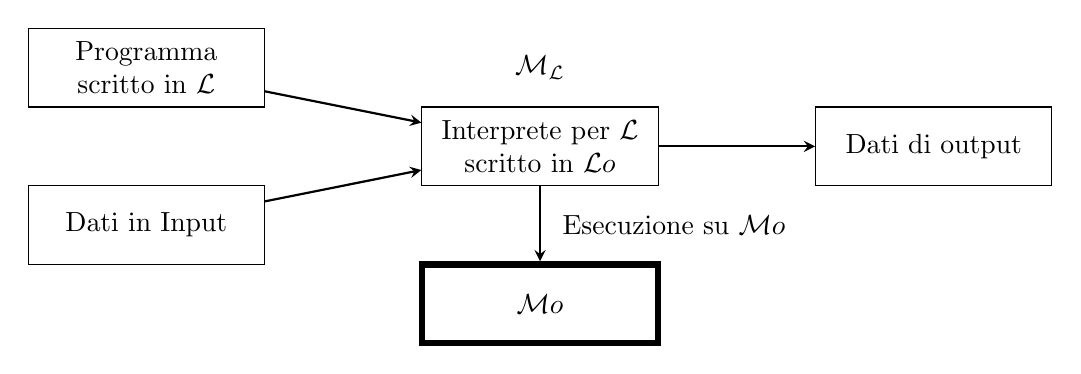
\begin{tikzpicture}[node distance=1cm]
        <TikZ code>
        
        \node (1) [rectangle, minimum width=3cm, minimum height=1cm, draw=black, align=center] {Programma \\ scritto in $\mathcal{L}$ \par};
        \node (2) [rectangle, yshift=-2cm, minimum width=3cm, minimum height=1cm, draw=black, align=center] {Dati in Input};
        \node (3) [rectangle, yshift=-1cm, xshift=5cm, minimum width=3cm, minimum height=1cm, draw=black, align=center] {Interprete per $\mathcal{L}$ \\ scritto in $\mathcal{L}o$ \par};
        \node (4) [rectangle, yshift=-1cm, xshift=10cm, minimum width=3cm, minimum height=1cm, draw=black, align=center] {Dati di output};
        
        \draw[arrow] (1) -- (3);
        \draw[arrow] (2) -- (3);
        \draw[arrow] (3) -- (4);
        
        \node (ML) [above of=3] {$\mathcal{M_L}$};
        \node (5) [rectangle, below of=3, yshift=-1cm, minimum width=3cm, minimum height=1cm, line width=2.25pt, draw=black, align=center] {$\mathcal{M}o$};
        
        \draw[arrow] (3) -- (5);
        \node (E) [below of=3, xshift=1.7cm] {Esecuzione su $\mathcal{M}o$};
        
    \end{tikzpicture}
    \begin{definizione}[Interprete]
        Un interprete per il linguaggio $\mathcal{L}$, scritto nel linguaggio $\mathcal{L}o$, è un programma che realizza una funzione parziale
        \[
            \mathcal{I_L}^{\mathcal{L}o}:(\mathcal{P}rog^{\mathcal{L}} \times \mathcal{D}) \longrightarrow \mathcal{D} \textnormal{ tale che } \mathcal{I_L}^{\mathcal{L}o}(\mathcal{P}_r^{\mathcal{L}}, Input)=\mathcal{P^L}(Input).
        \]
        Ovvero l'interprete "\textcolor{red}{calcola la corretta semantica}" del programma.
    \end{definizione}
    
    \newpage
    
    \subsection{Implementazione compilativa pura}
    in questa implementazione i programmi scritti nel linguaggio $\mathcal{L}$ vengono, prima di essere eseguiti, tradotti in programmi equivalenti scritti in linguaggio $\mathcal{L}o$ della mia macchina ospite.
    
    La differenza con L'implementazione interpretativa pura (\ref{Implementazione interpretativa pura}) è che: \\
    Prima L'Interprete eseguiva man mano che eseguiva il programma.
    
    ora il compilatore, prima traduce, e poi esegue
    
    \vspace{0.5cm}
    C'è quindi un programma particolare che si chiama \textcolor{red}{\textbf{compilatore}} che esegue la traduzione 
    \[ \mathcal{C}_{\mathcal{L,L}o}^{\mathcal{L}a} \]
    Il compilatore da $\mathcal{L}$ a $\mathcal{L}o$ scritto il $\mathcal{L}a$.
    
    \vspace{1cm}
    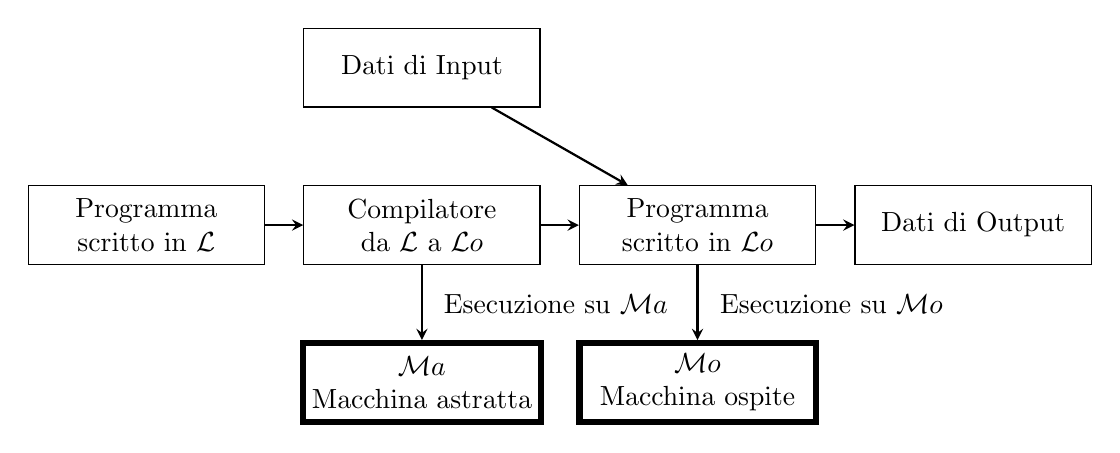
\begin{tikzpicture}
        <TikZ code>
        
        \node (1) [rectangle, minimum width=3cm, minimum height=1cm, draw=black, align=center] {Programma \\ scritto in $\mathcal{L}$ \par};
        \node (2) [rectangle, xshift=3.5cm, minimum width=3cm, minimum height=1cm, draw=black, align=center] {Compilatore \\ da $\mathcal{L}$ a $\mathcal{L}o$ \par};
        \node (3) [rectangle, xshift=7cm, minimum width=3cm, minimum height=1cm, draw=black, align=center] {Programma \\ scritto in $\mathcal{L}o$ \par};
        \node (4) [rectangle, xshift=10.5cm, minimum width=3cm, minimum height=1cm, draw=black, align=center] {Dati di Output};
        
        \draw[arrow] (1) -- (2);
        \draw[arrow] (2) -- (3);
        \draw[arrow] (3) -- (4);
        
        \node (I) [rectangle, above of=2, yshift=1cm, minimum width=3cm, minimum height=1cm, draw=black, align=center] {Dati di Input};
        
        \draw[arrow] (I) -- (3);
        
        \node (5) [rectangle, below of=2, yshift=-1cm, minimum width=3cm, minimum height=1cm, line width=2.25pt, draw=black, align=center] {$\mathcal{M}a$ \\ Macchina astratta \par};
        \node (6) [rectangle, below of=3, yshift=-1cm, minimum width=3cm, minimum height=1cm, line width=2.25pt, draw=black, align=center] {$\mathcal{M}o$ \\ Macchina ospite \par};
        
        \draw[arrow] (2) -- (5);
        \draw[arrow] (3) -- (6);
        
        \node [below of=2, xshift=1.7cm] {Esecuzione su $\mathcal{M}a$};
        \node [below of=3, xshift=1.7cm] {Esecuzione su $\mathcal{M}o$};
        
    \end{tikzpicture}
    \begin{definizione}[Compilatore]
        Un compilatore da $\mathcal{L}$ a $\mathrm{L}o$ è un programma che realizza una funzione
        \[ \mathcal{C}_{\mathcal{L,L}o}:\mathcal{P}rog^{\mathcal{L}} \longrightarrow \mathcal{P}rog^{\mathcal{L}o} \]
        tale che, dato un programma $\mathcal{P}_r^{\mathcal{L}}$, se
        \[ \mathcal{C}_{\mathcal{L,L}o}(\mathcal{P}_r^{\mathcal{L}})=\mathcal{P}_rc^{\mathcal{L}o} \]
        allora, per ogni $Input \in D^5$
        \[ \mathcal{P^L}(Input)=\mathcal{P}c^{\mathcal{L}o}(Input).
        \]
    \end{definizione}
    
    \newpage
    
    \subsection{Compilatore o Interpretatore?}
    \subsubsection{Implementazione interpretativa pura:}
    Ha sicuramente un difetto,
    \begin{itemize}
        \item \textbf{scarsa efficienza} della macchina $\mathcal{M_L}$. \\
        Perché ai tempi di esecuzione vanno aggiunti i tempi necessari alla decodifica.
    \end{itemize}
    Tuttavia l'implementazione interpretativa pura ha anche degli aspetti molto positivi:
    \begin{itemize}
        \item \textbf{Ha un'ottima flessibilità}: permette di interagire con l'esecuzione del programma
        \item \textbf{È più facile da realizzare}
        \item \textbf{Occupa meno memoria} (non viene effettivamente generato codice da memorizzare)
    \end{itemize}
    
    \subsubsection{Implementazione compilativa pura:}
    Sono un po' l'opposto dell'intrpretativa:
    \begin{itemize}
        \item difficile data la lontananza fra $\mathcal{L}$ e $\mathcal{L}o$
        \item buona efficienza
        \begin{enumerate}
            \item Il costo di decodifica è a carico del compilatore
            \item ogni istruzione è tradotta una sola volta
        \end{enumerate}
        \item scarsa flessibilità 
        \item c'è una perdita di informazione sulla struttura del programma sorgente, ovvero quando eseguo il programma scritto in $\mathcal{L}o$ se si manifesta un errore dinamico non è facile capire dove sta l'errore nel programma sorgente
        \item occupazione di memoria da parte del codice prodotto
    \end{itemize}
    
    \newpage
    
    \subsection{Nel caso reale}
    Nel caso reale \textbf{entrambe le due componenti coesistono}.
    
    Non si trovano mai implementazioni solo compilative o solo interpretative.
    
    \subsubsection{Implementazioni di tipo Interpretativo}
    L'interprete della macchina intermedia $\mathcal{M}_{\mathcal{L}i}$ è sostanzialmente diverso dall'interprete della macchina ospite $\mathcal{M}_o$
    
    \vspace{1cm}
    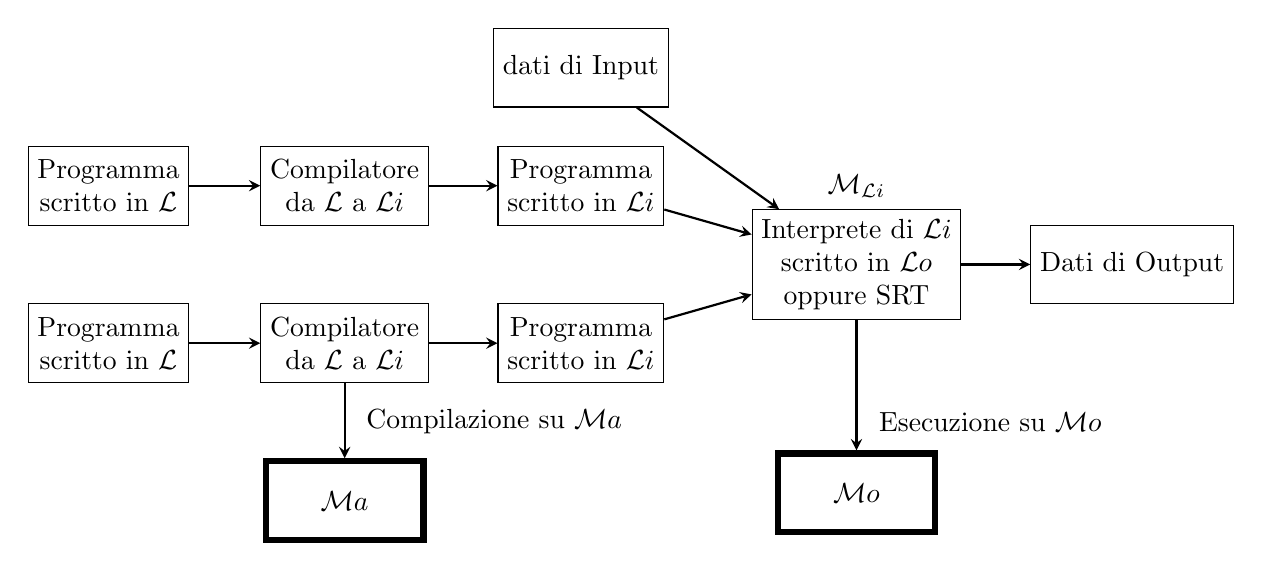
\begin{tikzpicture}
        <TikZ code>
        
        \node (1) [rectangle, minimum width=2cm, minimum height=1cm, draw=black, align=center] {Programma \\ scritto in $\mathcal{L}$};
        \node (2) [rectangle, yshift=-2cm, minimum width=2cm, minimum height=1cm, draw=black, align=center] {Programma \\ scritto in $\mathcal{L}$};
        \node (3) [rectangle, xshift=3cm, minimum width=2cm, minimum height=1cm, draw=black, align=center] {Compilatore \\ da $\mathcal{L}$ a $\mathcal{L}i$};
        \node (4) [rectangle, xshift=3cm, yshift=-2cm, minimum width=2cm, minimum height=1cm, draw=black, align=center] {Compilatore \\ da $\mathcal{L}$ a $\mathcal{L}i$};
        
        \draw[arrow] (1) -- (3);
        \draw[arrow] (2) -- (4);
        
        \node (5) [rectangle, xshift=6cm, minimum width=2cm, minimum height=1cm, draw=black, align=center] {Programma \\ scritto in $\mathcal{L}i$};
        \node (6) [rectangle, xshift=6cm, yshift=-2cm, minimum width=2cm, minimum height=1cm, draw=black, align=center] {Programma \\ scritto in $\mathcal{L}i$};
        
        \draw[arrow] (3) -- (5);
        \draw[arrow] (4) -- (6);
        
        \node (7) [rectangle, xshift=9.5cm, yshift=-1cm, minimum width=2cm, minimum height=1cm, draw=black, align=center] {Interprete di $\mathcal{L}i$  \\ scritto in $\mathcal{L}o$ \\ oppure SRT \par};
        
        \draw[arrow] (5) -- (7);
        \draw[arrow] (6) -- (7);
        
        \node (I) [rectangle, xshift=6cm, yshift=1.5cm, minimum width=2cm, minimum height=1cm, draw=black, align=center] {dati di Input};
        
        \node (8) [rectangle, xshift=13cm, yshift=-1cm, minimum width=2cm, minimum height=1cm, draw=black, align=center] {Dati di Output};
        
        \draw[arrow] (7) -- (8);
        \draw[arrow] (I) -- (7);
        
        \node (MLi) [above of=7] {$\mathcal{M}_{\mathcal{L}i}$};
        \node (MA) [rectangle, below of=4, yshift=-1cm, minimum width=2cm, minimum height=1cm, draw=black, line width=2.25pt, align=center] {$\mathcal{M}a$};
        \node (MO) [rectangle, below of=7, yshift=-1.9cm, minimum width=2cm, minimum height=1cm, draw=black, line width=2.25pt, align=center] {$\mathcal{M}o$};
        
        \draw[arrow] (4) -- (MA);
        \draw[arrow] (7) -- (MO);
        
        \node (CMA) [below of=4, xshift=1.9cm] {Compilazione su $\mathcal{M}a$};
        \node (EMO) [below of=7, xshift=1.7cm, yshift=-1cm] {Esecuzione su $\mathcal{M}o$};
        
    \end{tikzpicture}
    
    \paragraph{Esempio: Java}
    
    \verb| |\\
    
    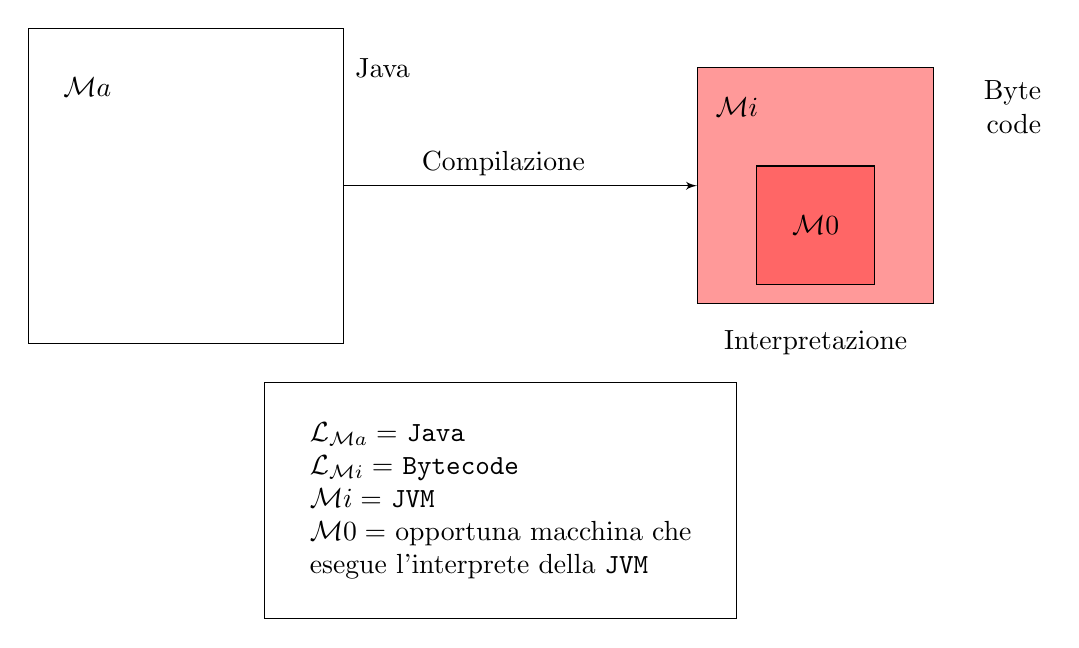
\begin{tikzpicture}
        <TikZ code>
        \node (Java) [rectangle, minimum width=4cm, minimum height=4cm, draw=black] {};
        \node (MAt) [xshift=-1.25cm, yshift=1.25cm] {$\mathcal{M}a$};
        \node (Jt) [xshift=2.5cm, yshift=1.5cm] {Java};
        \node (Bc) [rectangle, xshift=8cm, minimum width=3cm, minimum height=3cm, draw=black, fill=red!40] {};
        
        \node (Mi) [above of=Bc, xshift=-1cm] {$\mathcal{M}i$};
        \node (Bct) [right of=Bc, yshift=1cm, xshift=1.5cm, align=right] {Byte \\ code \par};
        \node (M0) [rectangle, minimum width=1.5cm, minimum height=1.5cm, below of=Bc, yshift=0.5cm, draw=black, fill=red!60] {$\mathcal{M}0$};
        \node (I) [below of=M0, yshift=-0.5cm] {Interpretazione};
        
        \path [line] (Java) -- node [text width=2.5cm,midway,above ] 
        {Compilazione} (Bc);

        \node (S) [rectangle, xshift=4cm, yshift=-4cm, minimum width=6cm, minimum height=3cm, draw=black, align=left] {$\mathcal{L}_{\mathcal{M}a} = $ \verb|Java| \\ $\mathcal{L}_{\mathcal{M}i} = $ \verb|Bytecode| \\ $\mathcal{M}i = $ \verb|JVM| \\ $\mathcal{M}0 = $ opportuna macchina che \\ esegue l'interprete della \verb|JVM| \par};
        
        
    \end{tikzpicture}
    
    
    \newpage
    \subsubsection{Implementazione di tipo compilativo}
    L'interprete della macchina intermedia $\mathcal{M}_{\mathcal{L}i}$ = interprete della macchina ospite + opportuni meccanismi (SRT - Supporto a Run Time)
    
    \vspace{0.1cm}
    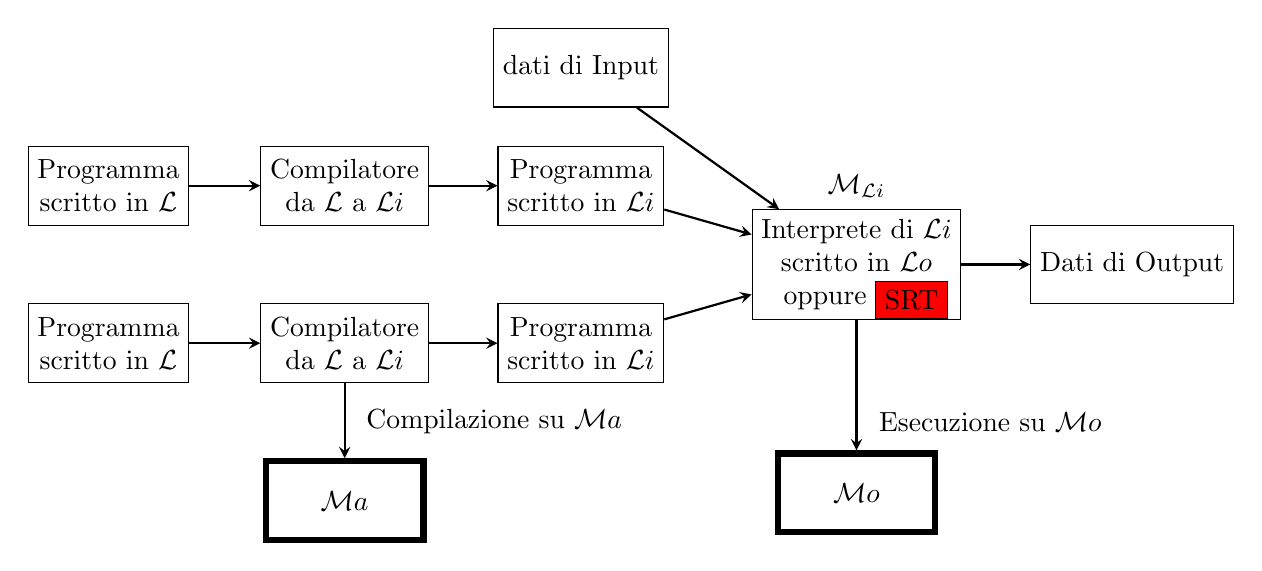
\begin{tikzpicture}
        <TikZ code>
        
        \node (1) [rectangle, minimum width=2cm, minimum height=1cm, draw=black, align=center] {Programma \\ scritto in $\mathcal{L}$};
        \node (2) [rectangle, yshift=-2cm, minimum width=2cm, minimum height=1cm, draw=black, align=center] {Programma \\ scritto in $\mathcal{L}$};
        \node (3) [rectangle, xshift=3cm, minimum width=2cm, minimum height=1cm, draw=black, align=center] {Compilatore \\ da $\mathcal{L}$ a $\mathcal{L}i$};
        \node (4) [rectangle, xshift=3cm, yshift=-2cm, minimum width=2cm, minimum height=1cm, draw=black, align=center] {Compilatore \\ da $\mathcal{L}$ a $\mathcal{L}i$};
        
        \draw[arrow] (1) -- (3);
        \draw[arrow] (2) -- (4);
        
        \node (5) [rectangle, xshift=6cm, minimum width=2cm, minimum height=1cm, draw=black, align=center] {Programma \\ scritto in $\mathcal{L}i$};
        \node (6) [rectangle, xshift=6cm, yshift=-2cm, minimum width=2cm, minimum height=1cm, draw=black, align=center] {Programma \\ scritto in $\mathcal{L}i$};
        
        \draw[arrow] (3) -- (5);
        \draw[arrow] (4) -- (6);
        
        \node (7) [rectangle, xshift=9.5cm, yshift=-1cm, minimum width=2cm, minimum height=1cm, draw=black, align=center] {Interprete di $\mathcal{L}i$  \\ scritto in $\mathcal{L}o$ \\ oppure SRT \par};
        
        \draw[arrow] (5) -- (7);
        \draw[arrow] (6) -- (7);
        
        \node (I) [rectangle, xshift=6cm, yshift=1.5cm, minimum width=2cm, minimum height=1cm, draw=black, align=center] {dati di Input};
        
        \node (8) [rectangle, xshift=13cm, yshift=-1cm, minimum width=2cm, minimum height=1cm, draw=black, align=center] {Dati di Output};
        
        \draw[arrow] (7) -- (8);
        \draw[arrow] (I) -- (7);
        
        \node (MLi) [above of=7] {$\mathcal{M}_{\mathcal{L}i}$};
        \node (MA) [rectangle, below of=4, yshift=-1cm, minimum width=2cm, minimum height=1cm, draw=black, line width=2.25pt, align=center] {$\mathcal{M}a$};
        \node (MO) [rectangle, below of=7, yshift=-1.9cm, minimum width=2cm, minimum height=1cm, draw=black, line width=2.25pt, align=center] {$\mathcal{M}o$};
        
        \draw[arrow] (4) -- (MA);
        \draw[arrow] (7) -- (MO);
        
        \node (CMA) [below of=4, xshift=1.9cm] {Compilazione su $\mathcal{M}a$};
        \node (EMO) [below of=7, xshift=1.7cm, yshift=-1cm] {Esecuzione su $\mathcal{M}o$};
        
        \node (SRT) [rectangle, below of=7, yshift=0.55cm, xshift=0.7cm, draw=black, fill=red] {SRT};
        
        
    \end{tikzpicture}
    
    \paragraph{Esempio: C}
    
    \verb| |\\
    
    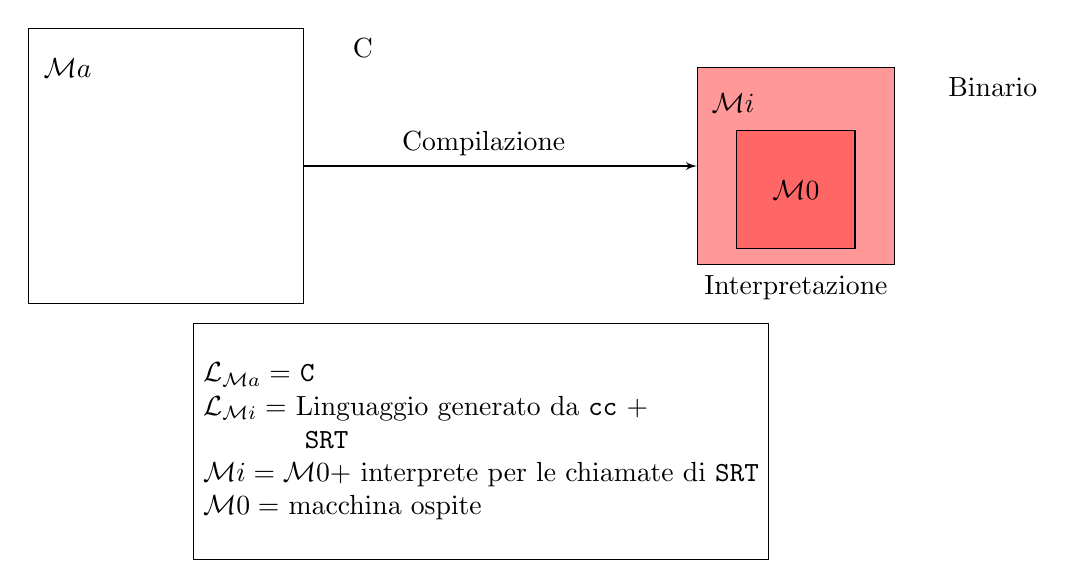
\begin{tikzpicture}
        <TikZ code>
        \node (Java) [rectangle, minimum width=3.5cm, minimum height=3.5cm, draw=black] {};
        \node (MAt) [xshift=-1.25cm, yshift=1.25cm] {$\mathcal{M}a$};
        \node (Jt) [xshift=2.5cm, yshift=1.5cm] {C};
        \node (Bc) [rectangle, xshift=8cm, minimum width=2.5cm, minimum height=2.5cm, draw=black, fill=red!40] {};
        
        \node (Mi) [above of=Bc, xshift=-0.8cm, yshift=-0.2cm] {$\mathcal{M}i$};
        \node (Bct) [right of=Bc, yshift=1cm, xshift=1.5cm, align=right] {Binario};
        \node (M0) [rectangle, minimum width=1.5cm, minimum height=1.5cm, below of=Bc, yshift=0.7cm, draw=black, fill=red!60] {$\mathcal{M}0$};
        \node (I) [below of=M0, yshift=-0.25cm] {Interpretazione};
        
        \path [line] (Java) -- node [text width=2.5cm,midway,above ] 
        {Compilazione} (Bc);

        \node (S) [rectangle, xshift=4cm, yshift=-3.5cm, minimum width=6cm, minimum height=3cm, draw=black, align=left] {$\mathcal{L}_{\mathcal{M}a} = $ \verb|C| \\
        $\mathcal{L}_{\mathcal{M}i} = $ Linguaggio generato da \verb|cc| $+$ \\ \verb|       SRT|  \\
        $\mathcal{M}i = \mathcal{M}0+$ interprete per le chiamate di \verb|SRT| \\
        $\mathcal{M}0 = $ macchina ospite };

    \end{tikzpicture}
    
    \subsection{Cosa compilare e cosa interpretare}
    Di base si tende a:
    \begin{itemize}
        \item tradurre i costrutti di $\mathcal{L}$ che sono simili a quelli di $\mathcal{L}o$;
        \item simulare (interpretazione) per gli altri.
    \end{itemize}
    
    \begin{tabular}{|c|c|}
        \hline
        Soluzione di tipo Compilativo & Soluzione di tipo interpretativo \\ \hline
        privilegia \textcolor{green}{\textbf{l'efficienze}} & privilegia \textcolor{red}{flessibilità e portabilità} \\ \hline
    \end{tabular}
    
    \section{È sempre possibile realizzare compilatore e l'interprete?}
    L'interprete è scritto in linguaggio ospite $\mathcal{L}_{osp}$ esegue il linguaggio sorgente $\mathcal{L}_{srg}$. \\
    Il compilatore è scritto in linguaggio ospite $\mathcal{L}_{osp}$ e traduce $\mathcal{L}_{srg}$ in $\mathcal{L}_{dest}$.
    
    Il compilatore preserva la semantica del programma tradotto, quindi preserva l'insieme delle funzioni che il linguaggio $\mathcal{L}_{srg}$ può calcolare.
    
    $\Rightarrow$ è necessario che $\mathcal{L}_{dest}$ sia non meno espressivo, potente almeno come $\mathcal{L}_{srg}$ 
    
    \subsection{Turing-completezza}
    \begin{definizione}[Turing-completezza]
        Un linguaggio viene detto \textit{Touring-completo} se calcola tutte le funzioni matematiche che possono essere calcolate con una macchina di Turing.
    \end{definizione}
    In questo corso però vedremo formalismi/linguaggi molto meno espressivi ma utili perché gli algoritmi relativi sono efficienti:
    \begin{multicols}{2}
    \begin{itemize}
        \item Automi finiti (analizzatori lessicali)
        \item Automi a pila (analizzatori sintattici)
    \end{itemize}
    \end{multicols}
    
    \subsection{come viene generato un compilatore}
    Come facciamo a costruire fisicamente un compilatore? ci sono degli strumenti automatici o semi-automatici che possono essere utilizzati.
    \begin{itemize}
        \item Lex (generatore di analizzatori lessicali) \\
        Parte da una opportuna specifica di com'è fatto il linguaggio di programmazione in oggetto e in modo automatico produce uno scanner che ci dice se il lessico usato nel programma è corretto oppure no.
        \item Yacc (generatore di analizzatori sintattici) \\
        Parte da un file con la specifica della grammatica del linguaggio di programmazione che stiamo usando per produrre un \textit{parser} ovvero un analizzatore sintattico, che preso in input un programma ci dice se le frasi utilizzate sono sintatticamente corrette oppure no.
    \end{itemize}
    
    \subsection{Bootstrapping}
    Come è possibile costruire compilatori con altri compilatori.
    
    % \subsubsection{Esempio: Pascal}
    \textbf{Esempio: Pascal} 
    
    I primi ambienti Pascal includevano:
    \begin{itemize}
        \item un compilatore in Pascal da Pascal a P-code: $\mathcal{C}^{Pascal}{_{Pascal, P-code}}$
        \item lo stesso compilatore tradotto in P-code: $\mathcal{C}^{P-code}{_{Pascal, P-code}}$
        \item un interprete per P-code, scritto in Pascal: $\mathcal{I}^{Pascal}{_{P-code}}$
    \end{itemize}
    \newpage
    Per poter avere un'implementazione locale su di una specifica macchina ospite $\mathcal{M}o$ era necessario produrre una traduzione dell'interprete $\mathcal{I}^{Pascal}{_{P-code}}$ nel linguaggio $\mathcal{M}o$
    
    \[\mathcal{I}^{\mathcal{L}o}{_{P-code}}\]
    
    Bisognava dunque eseguire su $\mathcal{M}o$ un programma $P$ in Pascal su dati $x$:
    \begin{align*}
        & \mathcal{I}^{\mathcal{L}o}{_{P-code}}(\mathcal{C}^{P-code}{_{Pascal, P-code}}, P) = P' \textnormal{ scritto in P-code } \\
        & \mathcal{I}^{\mathcal{L}o}{_{P-code}}(P', x) = \textnormal{ risultato vuoto }
    \end{align*}
    Si può fare di meglio però. \\
    Si può migliorare l'efficienza utilizzando un compilatore scritto in $\mathcal{L}o$
    
    Da $\mathcal{C}^{P-code}{_{Pascal, P-code}} \Longrightarrow \mathcal{C}^{Pascal}{_{Pascal, \mathcal{L}o}}$ \\
    Abbiamo quindi:
    \begin{itemize}
        \item $\mathcal{C}^{Pascal}{_{Pascal, P-code}}$
        \item $\mathcal{C}^{P-code}{_{Pascal, P-code}}$
        \item $\mathcal{I}^{Pascal}{_{P-code}}$
        \item $\mathcal{I}^{\mathcal{L}o}{_{P-code}}$
        \item $\mathcal{C}^{Pascal}{_{Pascal, \mathcal{L}o}}$
    \end{itemize}
    
    \textcolor{red}{\textbf{Bootstrapping}}
    \begin{align*}
         & \mathcal{I}^{\mathcal{L}o}{_{P-code}}(\mathcal{C}^{P-code}{_{Pascal, P-code}},\mathcal{C}^{Pascal}{_{Pascal, \mathcal{L}o}}) = \mathcal{C}^{P-code}{_{Pascal, \mathcal{L}o}} \\
         & \mathcal{I}^{\mathcal{L}o}{_{P-code}}(\mathcal{C}^{P-code}{_{Pascal, \mathcal{L}o}},\mathcal{C}^{Pascal}{_{Pascal, \mathcal{L}o}}) = \mathcal{C}^{\textcolor{red}{\mathcal{L}o}}{_{Pascal, \mathcal{L}o}}
    \end{align*}

\end{document}
